\section{Results}
\label{sec:results}

\subsection{Genetic Correlation}
\label{sub:psych_genetic_correlation}

Foremost, the genetic correlations betwee impulsive aggression and depressive symptomes is remarkably high ($r_g=0.6741$, $SE=0.0919$, $p=2.2326e-13$).
This high correlation is also reflected in a subjects diagnosed with a major depression ($r_g=0.4134$, $SE=0.1212$, $p=6e-04$).
In contrast, correlations between impulsive aggression and Bipolar disorder did not reached significant levels ($r_g=0.1192$, $SE=0.0949$, $p=0.2091$), and genetic correlations with Schizophrenia, while significant, was not of large effect ($r_g=0.161$, $SE=0.0566$, $p=0.0045$).


In contrast to impulsive aggression, correlations between risk taking and Bipolar ($r_g=0.2561$, $SE=0.0606$, $p=2.4034e-05$), as well as Schizophrenia ($r_g=0.232$, $SE=0.0431$, $p=7.3554e-08$) remain significant after adjusting for multiple testing.
In addition, while genetic correlations were highly significant between aggression and depression, genetic correlations between risk raking, depressive symptomes ($r_g=0.0856$, $SE=0.0687$, $p=0.2129$) as well as MD ($r_g=0.0028$, $SE=0.0853$, $p=0.974$) were small and did not pass the multple testing thershold.


\begin{figure}[htpb]
  \centering
  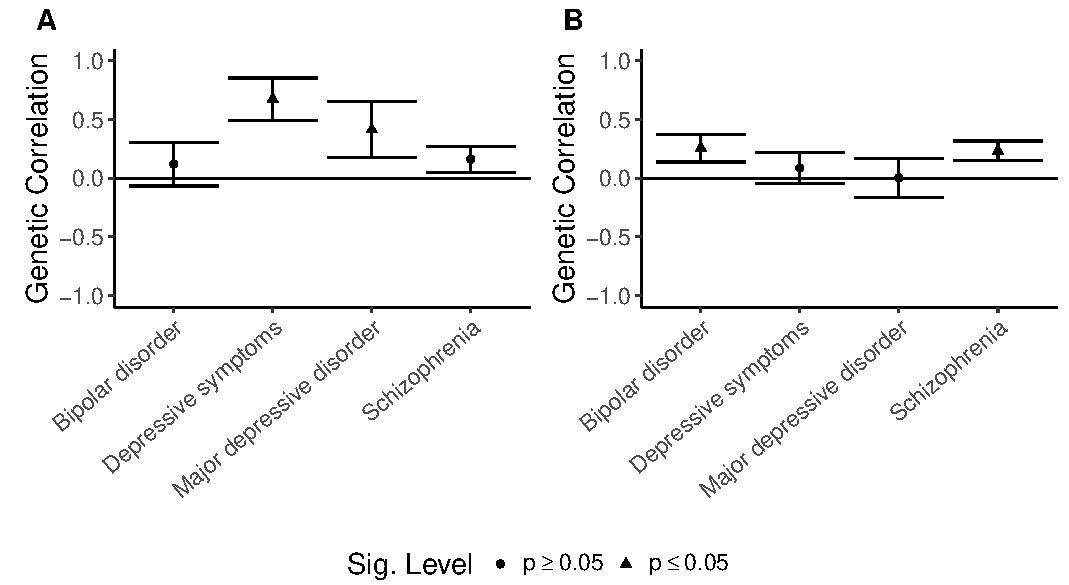
\includegraphics[width=0.8\linewidth]{figures/combined_corr.pdf}
  \caption{Genetic correlations between impulsive aggression and risk taking with selected psychiatric disorders.
    The error bars display the 95\% confidence intervals for each pairwise genetic correlations.
    Significance levels after multiple testing correction are displayed in form of a dot ($p\ge 0.05$) and triangle ($p\leq0.05$).
    (A) Genetic correlations between impulsive aggrsesion and psychiatric disorders. 
    (B) Genetic correlations between risk taking and psychiatric disorders.
  }\label{fig:figures/combined_corr}
\end{figure}

\subsection{Mendelian Randomization}
\label{sub:mendelian_randomization}

Applied MR-method suggest some indication for a causal effect on depressive symptomes on impulsive aggression (Figure~\ref{fig:overall_mr_effect}).
Noticable, all but one method indicate significant causal influence on aggression. 
Specifically, MR Egger, which represents a more conservative approch, shows not only non-significance but also displays a different direction of effect.
A possible explanation for this discrepency can be found in potential pleiotropic effects which might violate MR assumptions.
Inspection of the corresponding funnel plot (see Figure~\ref{fig:sensitivity}) suggest the some pleiotropic effects between selected SNPs and impulsive aggression.
However, other, more liberal method, do indicate a clear causal connection between depresssive symptomes and impulsive aggression.
This connection is further supported by an analysis of the MR of Major depressive disorder and aggression.
Corresponding to depressive symptomes, this analysis suggests that this sever metal disorder might cause an increase in aggressive behavior. 
In contrast, MR indicates no significant effect but demonstrats unity in regards to the direction of the effect across all used methods.
Inspection of the funnel plot further suggests neglectable pleiotropic effects which might violate the assumption.

\begin{figure}[htpb]
  \centering
  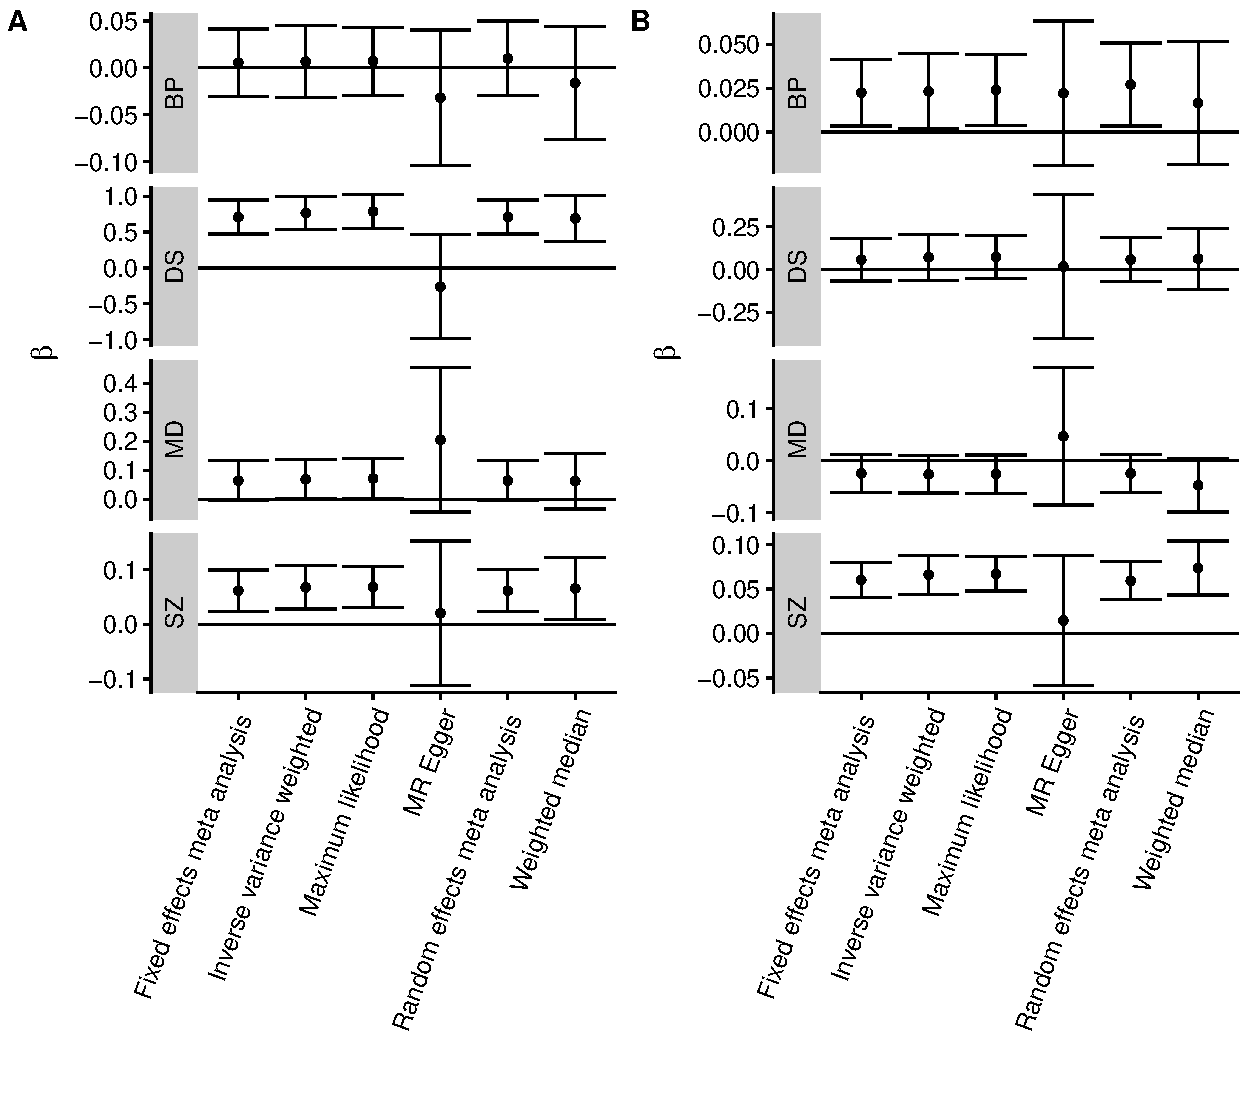
\includegraphics[width=0.9\linewidth]{figures/overall_mr_effect.pdf}
  \caption{Estimated causal effect of psychiatric disorders on impulsive aggression and risk taking.
    The effect size of the causal effect $\beta$ is displayed on the y-axis, while used Mendelian randomization methods are on the x-axis.
    SZ, Schizophrenia; MD, Major Depressive Disorder; DS, Depressive Symptomes; BP, Bipolar Disorder.
    (A) Effect of psychiatric disorders on impulsive aggression.
    (A) Effect of psychiatric disorders on risk taking.
  }\label{fig:overall_mr_effect}
\end{figure}

Further, there is some indication that SZ might cause an increase in aggressive behavior.
Similar to the analyses described above, all but MR-egger suggest a significant effect. 
However, in contrast to the previous described analysis there is very little evidence to support a violation of the underlying MR assumptions.
Thus making a causal connection between these two phenotypse more plausible.

In addition, to aggression MR in connection to risk taking only yield one potential causal relationship.
All used method, with the exception of MR-egger, suggest that Schizophrenia causes an increase in risk taking behavior.
Inspection of both funnel plots and intercept of the MR-egger regression coeffcient indicate no major violation of assumptions.


\begin{figure}[htpb]
  \centering
  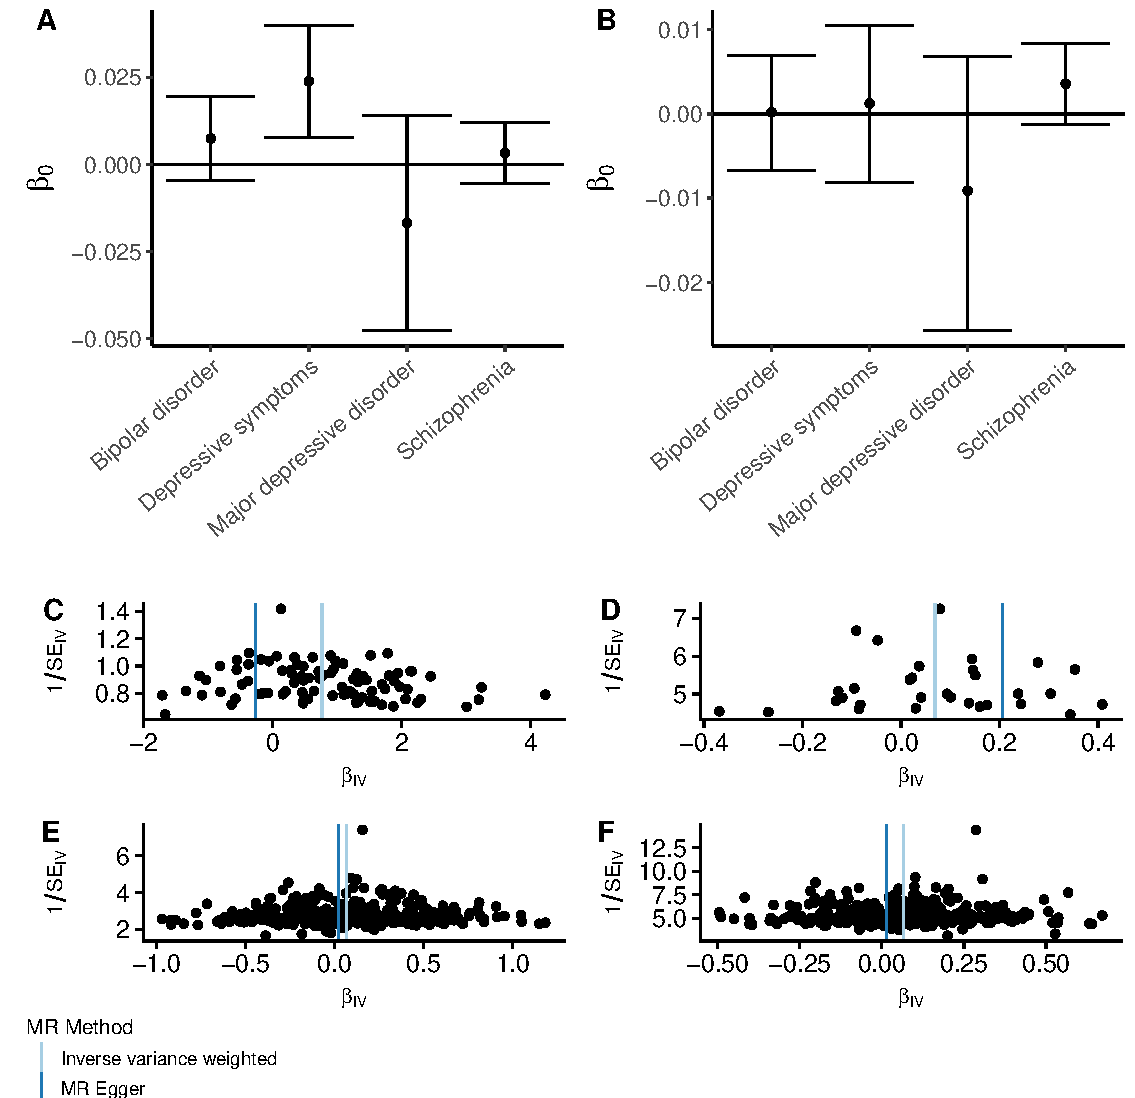
\includegraphics[width=0.9\linewidth]{figures/sensitvity_plot.pdf}
  \caption{Sensitivity analysis.
    (A) Displays the intercept of MR-egger regression for psychiatric disorders on impulsive aggression. The intercept is an indication of whether directional horizontal pleiotropy is driving the MR analysis.
    (B) The MR-egger regression intercept of psychiatric disorders on risk taking.
    (C) Funnel plot of Depressive symptoms on impulsive aggression. 
    (D) Funnel plot of MD on impulsive aggression. 
    (E) Funnel plot of SZ on impulsive aggression. 
    (F) Funnel plot of SZ on risk taking. 
    The intercept of both MR-egger and Inverse variance method are indicated with a vertical line.
    Errorbars indicate the 95\% confidence intervals.
  }\label{fig:sensitivity}
\end{figure}
